\section{Sistema multi-robot}
\setlength{\columnseprule}{0pt}
\onecolumn
Sea $\mathcal{S} = \{0, 1, \ldots, n\}$ el conjunto de robots móviles diferenciales.
\subsection{Comunicación}
La interacción entre agentes es modelada mediante un grafo dinámico $\mathcal{G}(t) = (\mathcal{S}, \mathcal{E}(t))$, donde $(i,j) \in \mathcal{E}(t)$ si y solo si $\|\mathbf{p}_i(t) - \mathbf{p}_j(t)\| \leq r_c$.

\setcounter{figure}{0}
\begin{figure}[H]
    \centering
    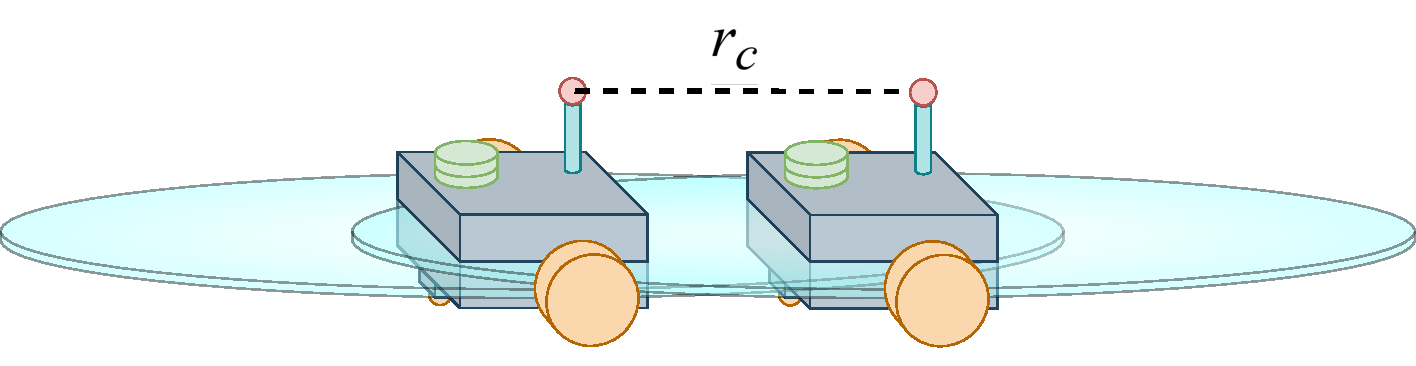
\includegraphics[width=0.5\linewidth]{Pics/comunicacionradio.pdf}
    \caption{Comunicación entre dos robots}
    \label{fig:lidar2}
\end{figure}